\documentclass[output=paper]{langsci/langscibook} 
\author{Sam Hellmuth\affiliation{University of York}}
\title{Contact and variation in Arabic intonation}
\abstract{Evidence is emerging of differences among Arabic dialects in their intonation patterns, along known parameters of variation in prosodic typology. Through a series of brief case studies, this chapter explores the hypothesis that variation in intonation in Arabic results from changes in the phonology of individual Arabic varieties, triggered by past (or present-day) speaker bilingualism. If correct, variation in intonation should reflect prosodic properties of the specific languages that a particular regional dialect has had contact with.}
\IfFileExists{../localcommands.tex}{
  % add all extra packages you need to load to this file 
\usepackage{graphicx}
\usepackage{tabularx}
\usepackage{amsmath} 
\usepackage{multicol}
\usepackage{lipsum}
\usepackage[stable]{footmisc}
\usepackage{adforn}
%%%%%%%%%%%%%%%%%%%%%%%%%%%%%%%%%%%%%%%%%%%%%%%%%%%%
%%%                                              %%%
%%%           Examples                           %%%
%%%                                              %%%
%%%%%%%%%%%%%%%%%%%%%%%%%%%%%%%%%%%%%%%%%%%%%%%%%%%%
% remove the percentage signs in the following lines
% if your book makes use of linguistic examples
\usepackage{./langsci/styles/langsci-optional} 
\usepackage{./langsci/styles/langsci-lgr}
\usepackage{morewrites} 
%% if you want the source line of examples to be in italics, uncomment the following line
% \def\exfont{\it}

\usepackage{enumitem}
\newlist{furtherreading}{description}{1}
\setlist[furtherreading]{font=\normalfont,labelsep=\widthof{~},noitemsep,align=left,leftmargin=\parindent,labelindent=0pt,labelwidth=-\parindent}
\usepackage{phonetic}
\usepackage{chronosys,tabularx}
\usepackage{csquotes}
\usepackage[stable]{footmisc} 

\usepackage{langsci-bidi}
\usepackage{./langsci/styles/langsci-gb4e} 

  \makeatletter
\let\thetitle\@title
\let\theauthor\@author 
\makeatother

\newcommand{\togglepaper}[1][0]{ 
  \bibliography{../localbibliography}
  \papernote{\scriptsize\normalfont
    \theauthor.
    \thetitle. 
    To appear in: 
    Christopher Lucas and Stefano Manfredi (eds.),  
    Arabic and contact-induced language change
    Berlin: Language Science Press. [preliminary page numbering]
  }
  \pagenumbering{roman}
  \setcounter{chapter}{#1}
  \addtocounter{chapter}{-1}
}

\newfontfamily\Parsifont[Script=Arabic]{ScheherazadeRegOT_Jazm.ttf} 
\newcommand{\arabscript}[1]{\RL{\Parsifont #1}}
\newcommand{\textarabic}[1]{{\arabicfont #1}}

\newcommand{\textstylest}[1]{{\color{red}#1}}

\patchcmd{\mkbibindexname}{\ifdefvoid{#3}{}{\MakeCapital{#3}
}}{\ifdefvoid{#3}{}{#3 }}{}{\AtEndDocument{\typeout{mkbibindexname could
not be patched.}}}

%command for italic r with dot below with horizontal correction to put the dot in the prolongation of the vertical stroke
%for some reason, the dot is larger than expected, so we explicitly reduce the font size (to \small)
%for the time being, the font is set to an absolute value. To be more robust, a relative reduction would be better, but this might not be required right now
\newcommand{\R}{r\kern-.05ex{\small{̣}}\kern.05ex}


\DeclareLabeldate{%
    \field{date}
    \field{year}
    \field{eventdate}
    \field{origdate}
    \field{urldate}
    \field{pubstate}
    \literal{nodate}
}

\renewbibmacro*{addendum+pubstate}{% Thanks to https://tex.stackexchange.com/a/154367 for the idea
  \printfield{addendum}%
  \iffieldequalstr{labeldatesource}{pubstate}{}
  {\newunit\newblock\printfield{pubstate}}
}
 
  %% hyphenation points for line breaks
%% Normally, automatic hyphenation in LaTeX is very good
%% If a word is mis-hyphenated, add it to this file
%%
%% add information to TeX file before \begin{document} with:
%% %% hyphenation points for line breaks
%% Normally, automatic hyphenation in LaTeX is very good
%% If a word is mis-hyphenated, add it to this file
%%
%% add information to TeX file before \begin{document} with:
%% %% hyphenation points for line breaks
%% Normally, automatic hyphenation in LaTeX is very good
%% If a word is mis-hyphenated, add it to this file
%%
%% add information to TeX file before \begin{document} with:
%% \include{localhyphenation}
\hyphenation{
affri-ca-te
affri-ca-tes
com-ple-ments
homo-phon-ous
start-ed
Meso-potam-ian
morpho-phono-logic-al-ly
morpho-phon-em-ic-s
Palestin-ian
re-present-ed
Ki-nubi
ḥawār-iyy-ūn
archa-ic-ity
fuel-ed
de-velop-ment
pros-od-ic
Arab-ic
in-duced
phono-logy
possess-um
possess-ive-s
templ-ate
spec-ial
espec-ial-ly
nat-ive
pass-ive
clause-s
potent-ial-ly
Lusignan
commun-ity
tobacco
posi-tion
Cushit-ic
Middle
with-in
re-finit-iz-ation
langu-age-s
langu-age
diction-ary
glossary
govern-ment
eight
counter-part
nomin-al
equi-valent
deont-ic
ana-ly-sis
Malt-ese
un-fortun-ate-ly
scient-if-ic
Catalan
Occitan
ḥammāl
cross-linguist-ic-al-ly
predic-ate
major-ity
ignor-ance
chrono-logy
south-western
mention-ed
borrow-ed
neg-ative
de-termin-er
European
under-mine
detail
Oxford
Socotra
numer-ous
spoken
villages
nomad-ic
Khuze-stan
Arama-ic
Persian
Ottoman
Ottomans
Azeri
rur-al
bi-lingual-ism
borrow-ing
prestig-ious
dia-lects
dia-lect
allo-phone
allo-phones
poss-ible
parallel
parallels
pattern
article
common-ly
respect-ive-ly
sem-antic
Moroccan
Martine
Harrassowitz
Grammatic-al-ization
grammatic-al-ization
Afro-asiatica
Afro-asiatic
continu-ation
Semit-istik
varieties
mono-phthong
mono-phthong-ized
col-loquial
pro-duct
document-ary
ex-ample-s
ex-ample
termin-ate
element-s
Aramaeo-grams
Centr-al
idioms
Arab-ic
Dadan-it-ic
sub-ordin-ator
Thamud-ic
difficult
common-ly
Revue
Bovingdon
under
century
attach
attached
bundle
graph-em-ic
graph-emes
cicada
contrast-ive
Corriente
Andalusi
Kossmann
morpho-logic-al
inter-action
dia-chroniques
islámica
occid-ent-al-ismo
dialecto-logie
Reichert
coloni-al
Milton
diphthong-al
linguist-ic
linguist-ics
affairs
differ-ent
phonetic-ally
kilo-metres
stabil-ization
develop-ments
in-vestig-ation
Jordan-ian
notice-able
level-ed
migrants
con-dition-al
certain-ly
general-ly
especial-ly
af-fric-ation
Jordan
counter-parts
com-plication
consider-ably
inter-dent-al
com-mun-ity
inter-locutors
com-pon-ent
region-al
socio-historical
society
simul-taneous
phon-em-ic
roman-ization
Classic-al
funeral
Kurmanji
pharyn-geal-ization
vocab-ulary
phon-et-ic
con-sonant
con-sonants
special-ized
latter
latters
in-itial
ident-ic-al
cor-relate
geo-graphic-al-ly
Öpengin
Kurd-ish
in-digen-ous
sunbul
Christ-ian
Christ-ians
sekin-în
fatala
in-tegration
dia-lect-al
Matras
morpho-logy
in-tens-ive
con-figur-ation
im-port-ant
com-plement
ḥaddād
e-merg-ence
Benjmamins
struct-ure
em-pir-ic-al
Orient-studien
Anatolia
American
vari-ation
Jastrow
Geoffrey
Yarshater
Ashtiany
Edmund
Mahnaz
En-cyclo-pædia
En-cyclo-paedia
En-cyclo-pedia
Leiden
dia-spora
soph-is-ic-ated
Sasan-ian
every-day
domin-ance
Con-stitu-tion-al
religi-ous
sever-al
Manfredi
re-lev-ance
re-cipi-ent
pro-duct-iv-ity
turtle
Morocco
ferman
Maghreb-ian
algérien
stand-ard
systems
Nicolaï
Mouton
mauritani-en
Gotho-burg-ensis
socio-linguist-ique
plur-al
archiv-al
Arab-ian
drop-ped
dihāt
de-velop-ed
ṣuḥbat
kitāba
kitābat
com-mercial
eight-eenth
region
Senegal
mechan-ics
Maur-itan-ia
Ḥassān-iyya
circum-cision
cor-relation
labio-velar-ization
vowel
vowels
cert-ain
īggīw
series
in-tegrates
dur-ative
inter-dent-als
gen-itive
Tuareg
tălămut
talawmāyət
part-icular
part-icular-ly
con-diment
vill-age
bord-er
polit-ical
Wiesbaden
Uni-vers-idad
Geuthner
typo-logie
Maur-itanie
nomades
Maur-itan-ian
dia-lecto-logy
Sahar-iennes
Uni-vers-ity
de-scend-ants
NENA-speak-ing
speak-ing
origin-al
re-captured
in-habit-ants
ethnic
minor-it-ies
drama-tic
local
long-stand-ing
regions
Nineveh
settle-ments
Ṣəndor
Mandate
sub-stitut-ing
ortho-graphy
re-fer-enced
origin-ate
twenti-eth
typ-ic-al-ly
Hobrack
never-the-less
character-ist-ics
character-ist-ic
masc-uline
coffee
ex-clus-ive-ly
verb-al
re-ana-ly-se-d
simil-ar-ities
de-riv-ation
im-pera-tive
part-iciple
dis-ambi-gu-ation
dis-ambi-gu-a-ing
phen-omen-on
phen-omen-a
traktar
com-mun-ity
com-mun-ities
dis-prefer-red
ex-plan-ation
con-struction
wide-spread
us-ual-ly
region-al
Bulut
con-sider-ation
afro-asia-tici
Franco-Angeli
Phono-logie
Volks-kundliche
dia-lectes
dia-lecte
select-ed
dis-appear-ance
media
under-stand-able
public-ation
second-ary
e-ject-ive
re-volu-tion
re-strict-ive
Gasparini
mount-ain
mount-ains
yellow
label-ing
trad-ition-al-ly
currently
dia-chronic
}
\hyphenation{
affri-ca-te
affri-ca-tes
com-ple-ments
homo-phon-ous
start-ed
Meso-potam-ian
morpho-phono-logic-al-ly
morpho-phon-em-ic-s
Palestin-ian
re-present-ed
Ki-nubi
ḥawār-iyy-ūn
archa-ic-ity
fuel-ed
de-velop-ment
pros-od-ic
Arab-ic
in-duced
phono-logy
possess-um
possess-ive-s
templ-ate
spec-ial
espec-ial-ly
nat-ive
pass-ive
clause-s
potent-ial-ly
Lusignan
commun-ity
tobacco
posi-tion
Cushit-ic
Middle
with-in
re-finit-iz-ation
langu-age-s
langu-age
diction-ary
glossary
govern-ment
eight
counter-part
nomin-al
equi-valent
deont-ic
ana-ly-sis
Malt-ese
un-fortun-ate-ly
scient-if-ic
Catalan
Occitan
ḥammāl
cross-linguist-ic-al-ly
predic-ate
major-ity
ignor-ance
chrono-logy
south-western
mention-ed
borrow-ed
neg-ative
de-termin-er
European
under-mine
detail
Oxford
Socotra
numer-ous
spoken
villages
nomad-ic
Khuze-stan
Arama-ic
Persian
Ottoman
Ottomans
Azeri
rur-al
bi-lingual-ism
borrow-ing
prestig-ious
dia-lects
dia-lect
allo-phone
allo-phones
poss-ible
parallel
parallels
pattern
article
common-ly
respect-ive-ly
sem-antic
Moroccan
Martine
Harrassowitz
Grammatic-al-ization
grammatic-al-ization
Afro-asiatica
Afro-asiatic
continu-ation
Semit-istik
varieties
mono-phthong
mono-phthong-ized
col-loquial
pro-duct
document-ary
ex-ample-s
ex-ample
termin-ate
element-s
Aramaeo-grams
Centr-al
idioms
Arab-ic
Dadan-it-ic
sub-ordin-ator
Thamud-ic
difficult
common-ly
Revue
Bovingdon
under
century
attach
attached
bundle
graph-em-ic
graph-emes
cicada
contrast-ive
Corriente
Andalusi
Kossmann
morpho-logic-al
inter-action
dia-chroniques
islámica
occid-ent-al-ismo
dialecto-logie
Reichert
coloni-al
Milton
diphthong-al
linguist-ic
linguist-ics
affairs
differ-ent
phonetic-ally
kilo-metres
stabil-ization
develop-ments
in-vestig-ation
Jordan-ian
notice-able
level-ed
migrants
con-dition-al
certain-ly
general-ly
especial-ly
af-fric-ation
Jordan
counter-parts
com-plication
consider-ably
inter-dent-al
com-mun-ity
inter-locutors
com-pon-ent
region-al
socio-historical
society
simul-taneous
phon-em-ic
roman-ization
Classic-al
funeral
Kurmanji
pharyn-geal-ization
vocab-ulary
phon-et-ic
con-sonant
con-sonants
special-ized
latter
latters
in-itial
ident-ic-al
cor-relate
geo-graphic-al-ly
Öpengin
Kurd-ish
in-digen-ous
sunbul
Christ-ian
Christ-ians
sekin-în
fatala
in-tegration
dia-lect-al
Matras
morpho-logy
in-tens-ive
con-figur-ation
im-port-ant
com-plement
ḥaddād
e-merg-ence
Benjmamins
struct-ure
em-pir-ic-al
Orient-studien
Anatolia
American
vari-ation
Jastrow
Geoffrey
Yarshater
Ashtiany
Edmund
Mahnaz
En-cyclo-pædia
En-cyclo-paedia
En-cyclo-pedia
Leiden
dia-spora
soph-is-ic-ated
Sasan-ian
every-day
domin-ance
Con-stitu-tion-al
religi-ous
sever-al
Manfredi
re-lev-ance
re-cipi-ent
pro-duct-iv-ity
turtle
Morocco
ferman
Maghreb-ian
algérien
stand-ard
systems
Nicolaï
Mouton
mauritani-en
Gotho-burg-ensis
socio-linguist-ique
plur-al
archiv-al
Arab-ian
drop-ped
dihāt
de-velop-ed
ṣuḥbat
kitāba
kitābat
com-mercial
eight-eenth
region
Senegal
mechan-ics
Maur-itan-ia
Ḥassān-iyya
circum-cision
cor-relation
labio-velar-ization
vowel
vowels
cert-ain
īggīw
series
in-tegrates
dur-ative
inter-dent-als
gen-itive
Tuareg
tălămut
talawmāyət
part-icular
part-icular-ly
con-diment
vill-age
bord-er
polit-ical
Wiesbaden
Uni-vers-idad
Geuthner
typo-logie
Maur-itanie
nomades
Maur-itan-ian
dia-lecto-logy
Sahar-iennes
Uni-vers-ity
de-scend-ants
NENA-speak-ing
speak-ing
origin-al
re-captured
in-habit-ants
ethnic
minor-it-ies
drama-tic
local
long-stand-ing
regions
Nineveh
settle-ments
Ṣəndor
Mandate
sub-stitut-ing
ortho-graphy
re-fer-enced
origin-ate
twenti-eth
typ-ic-al-ly
Hobrack
never-the-less
character-ist-ics
character-ist-ic
masc-uline
coffee
ex-clus-ive-ly
verb-al
re-ana-ly-se-d
simil-ar-ities
de-riv-ation
im-pera-tive
part-iciple
dis-ambi-gu-ation
dis-ambi-gu-a-ing
phen-omen-on
phen-omen-a
traktar
com-mun-ity
com-mun-ities
dis-prefer-red
ex-plan-ation
con-struction
wide-spread
us-ual-ly
region-al
Bulut
con-sider-ation
afro-asia-tici
Franco-Angeli
Phono-logie
Volks-kundliche
dia-lectes
dia-lecte
select-ed
dis-appear-ance
media
under-stand-able
public-ation
second-ary
e-ject-ive
re-volu-tion
re-strict-ive
Gasparini
mount-ain
mount-ains
yellow
label-ing
trad-ition-al-ly
currently
dia-chronic
}
\hyphenation{
affri-ca-te
affri-ca-tes
com-ple-ments
homo-phon-ous
start-ed
Meso-potam-ian
morpho-phono-logic-al-ly
morpho-phon-em-ic-s
Palestin-ian
re-present-ed
Ki-nubi
ḥawār-iyy-ūn
archa-ic-ity
fuel-ed
de-velop-ment
pros-od-ic
Arab-ic
in-duced
phono-logy
possess-um
possess-ive-s
templ-ate
spec-ial
espec-ial-ly
nat-ive
pass-ive
clause-s
potent-ial-ly
Lusignan
commun-ity
tobacco
posi-tion
Cushit-ic
Middle
with-in
re-finit-iz-ation
langu-age-s
langu-age
diction-ary
glossary
govern-ment
eight
counter-part
nomin-al
equi-valent
deont-ic
ana-ly-sis
Malt-ese
un-fortun-ate-ly
scient-if-ic
Catalan
Occitan
ḥammāl
cross-linguist-ic-al-ly
predic-ate
major-ity
ignor-ance
chrono-logy
south-western
mention-ed
borrow-ed
neg-ative
de-termin-er
European
under-mine
detail
Oxford
Socotra
numer-ous
spoken
villages
nomad-ic
Khuze-stan
Arama-ic
Persian
Ottoman
Ottomans
Azeri
rur-al
bi-lingual-ism
borrow-ing
prestig-ious
dia-lects
dia-lect
allo-phone
allo-phones
poss-ible
parallel
parallels
pattern
article
common-ly
respect-ive-ly
sem-antic
Moroccan
Martine
Harrassowitz
Grammatic-al-ization
grammatic-al-ization
Afro-asiatica
Afro-asiatic
continu-ation
Semit-istik
varieties
mono-phthong
mono-phthong-ized
col-loquial
pro-duct
document-ary
ex-ample-s
ex-ample
termin-ate
element-s
Aramaeo-grams
Centr-al
idioms
Arab-ic
Dadan-it-ic
sub-ordin-ator
Thamud-ic
difficult
common-ly
Revue
Bovingdon
under
century
attach
attached
bundle
graph-em-ic
graph-emes
cicada
contrast-ive
Corriente
Andalusi
Kossmann
morpho-logic-al
inter-action
dia-chroniques
islámica
occid-ent-al-ismo
dialecto-logie
Reichert
coloni-al
Milton
diphthong-al
linguist-ic
linguist-ics
affairs
differ-ent
phonetic-ally
kilo-metres
stabil-ization
develop-ments
in-vestig-ation
Jordan-ian
notice-able
level-ed
migrants
con-dition-al
certain-ly
general-ly
especial-ly
af-fric-ation
Jordan
counter-parts
com-plication
consider-ably
inter-dent-al
com-mun-ity
inter-locutors
com-pon-ent
region-al
socio-historical
society
simul-taneous
phon-em-ic
roman-ization
Classic-al
funeral
Kurmanji
pharyn-geal-ization
vocab-ulary
phon-et-ic
con-sonant
con-sonants
special-ized
latter
latters
in-itial
ident-ic-al
cor-relate
geo-graphic-al-ly
Öpengin
Kurd-ish
in-digen-ous
sunbul
Christ-ian
Christ-ians
sekin-în
fatala
in-tegration
dia-lect-al
Matras
morpho-logy
in-tens-ive
con-figur-ation
im-port-ant
com-plement
ḥaddād
e-merg-ence
Benjmamins
struct-ure
em-pir-ic-al
Orient-studien
Anatolia
American
vari-ation
Jastrow
Geoffrey
Yarshater
Ashtiany
Edmund
Mahnaz
En-cyclo-pædia
En-cyclo-paedia
En-cyclo-pedia
Leiden
dia-spora
soph-is-ic-ated
Sasan-ian
every-day
domin-ance
Con-stitu-tion-al
religi-ous
sever-al
Manfredi
re-lev-ance
re-cipi-ent
pro-duct-iv-ity
turtle
Morocco
ferman
Maghreb-ian
algérien
stand-ard
systems
Nicolaï
Mouton
mauritani-en
Gotho-burg-ensis
socio-linguist-ique
plur-al
archiv-al
Arab-ian
drop-ped
dihāt
de-velop-ed
ṣuḥbat
kitāba
kitābat
com-mercial
eight-eenth
region
Senegal
mechan-ics
Maur-itan-ia
Ḥassān-iyya
circum-cision
cor-relation
labio-velar-ization
vowel
vowels
cert-ain
īggīw
series
in-tegrates
dur-ative
inter-dent-als
gen-itive
Tuareg
tălămut
talawmāyət
part-icular
part-icular-ly
con-diment
vill-age
bord-er
polit-ical
Wiesbaden
Uni-vers-idad
Geuthner
typo-logie
Maur-itanie
nomades
Maur-itan-ian
dia-lecto-logy
Sahar-iennes
Uni-vers-ity
de-scend-ants
NENA-speak-ing
speak-ing
origin-al
re-captured
in-habit-ants
ethnic
minor-it-ies
drama-tic
local
long-stand-ing
regions
Nineveh
settle-ments
Ṣəndor
Mandate
sub-stitut-ing
ortho-graphy
re-fer-enced
origin-ate
twenti-eth
typ-ic-al-ly
Hobrack
never-the-less
character-ist-ics
character-ist-ic
masc-uline
coffee
ex-clus-ive-ly
verb-al
re-ana-ly-se-d
simil-ar-ities
de-riv-ation
im-pera-tive
part-iciple
dis-ambi-gu-ation
dis-ambi-gu-a-ing
phen-omen-on
phen-omen-a
traktar
com-mun-ity
com-mun-ities
dis-prefer-red
ex-plan-ation
con-struction
wide-spread
us-ual-ly
region-al
Bulut
con-sider-ation
afro-asia-tici
Franco-Angeli
Phono-logie
Volks-kundliche
dia-lectes
dia-lecte
select-ed
dis-appear-ance
media
under-stand-able
public-ation
second-ary
e-ject-ive
re-volu-tion
re-strict-ive
Gasparini
mount-ain
mount-ains
yellow
label-ing
trad-ition-al-ly
currently
dia-chronic
} 
  \togglepaper[1]%%chapternumber
}{}

\begin{document}
\maketitle 
 
 

 \section{Introduction}


 \subsection{Rationale}


The hypothesis explored in this chapter is that observed synchronic variation in \isi{intonation} across \ili{Arabic} dialects is contact-induced. In this scenario, differences between dialects would result from changes in the intonational phonology of individual varieties triggered by speaker \isi{bilingualism} in \ili{Arabic} and one or more other languages \citep{Lucas2015}, either in the past, or up to and including the present day. To achieve this, I outline a framework for analysis of variation in \isi{intonation} (§\ref{cross}), summarise recent research on the effects of \isi{bilingualism} on the intonational phonology of bilingual individuals and the languages they speak (§\ref{var}), and sketch the types of language contact scenario which may be relevant for \ili{Arabic} (§\ref{aravar}). In §\ref{araint} I present case studies of prosodic features which appear to be specific to a particular dialect, on current evidence at least, and discuss which of the potentially relevant contact languages might have served as the potential source of the feature in question, considering also possible endogenous (internal) sources of the change. The chapter closes (§\ref{closes}) with suggestions for \isi{future} research.


 
 \subsection{Cross-linguistic variation in intonation} \label{cross}


Any attempt to delimit the nature and scope of variation in \isi{intonation} depends on the model of intonational phonology adopted. The analyses explored in §\ref{araint} below are framed in the Autosegmental-Metrical (AM) theory of \isi{intonation} \citep{Ladd2008}, and the parameters of intonational variation explored are thus influenced by this choice. 

A basic debate in the analysis of \isi{intonation} is whether the primitives of the system are whole contours (defined over an intonational phrase), or some sub-component of those contours \citep{Ladd2008}. In AM theory, \isi{intonation} is modelled as interpolation of pitch between tonal targets; these tonal targets are the primitives of the system and are of two types: pitch accents are associated with the heads of metrical domains (e.g. stressed syllables), boundary tones are associated with the edges of metrical domains (e.g. prosodic phrases). In AM, tonal targets are transcribed using combinations of high (H) or low (L) targets, which reflect significant peaks and valleys, respectively, in the pitch contour of the utterance; association of these events to landmarks in the metrical structure is marked using ``*'' for pitch accents (associated with stressed syllables) and ``\%'' for boundary tones (associated with the right edge of prosodic phrases of different sizes). A typical AM analysis yields an inventory of the pitch accents and boundary tones needed to model the contours in a corpus of speech data, supported by a description of the observed contours (\citealt{JunFletcher2015}).

Ladd's (\citeyear{Ladd2008}) taxonomy of possible parameters of cross-linguistic variation in \isi{intonation} (based on \citealt{Wells1982}) envisages four broad (inter-related) categories of variation: systemic (differences in the inventory of pitch accents or boundary tones); semantic (differences in the meaning or function associated with a particular contour, pitch accent or boundary \isi{tone}); realisational (differences in the phonetic realisation of otherwise parallel pitch accents or boundary tones; and phonotactic (differences in the distribution of pitch accents and boundary tones, or in their association to metrical structure). 

Comparison of AM analyses across a typologically distinct set of languages (\citealt{Jun2005,Jun2015}) has highlighted systematic cross-linguistic variation of a systemic and/or phonotactic nature, in terms of prosodic phrasing (with relatively smaller or larger domains involved in structural organization of \isi{intonation} patterns), the distribution of tonal events \isi{relative} to prosodic constituents (marking either the edges or the metrical heads of phrases or both), and the size and composition of the inventory of tonal events regularly observed (pitch accents and boundary tones). There is also a large body of research on cross-linguistic variation in the phonetic realisation of pitch accents, in particular on peak alignment (\citealt{AttererLadd2004}; \citealt{Ladd2006}) and scaling (\citealt{LaddMorton1997}), confirming the existence of realisational cross-linguistic variation. The most advanced work on semantic variation to date has been on \ili{Romance} languages, facilitated by a concerted effort to develop descriptions of these languages' \isi{intonation} patterns within a common annotation system (\citealt{FrotaPrieto2015}). 

For \ili{Arabic}, evidence is emerging of variation along similar lines. Recent review articles have highlighted clear differences in the size and composition of the inventory of pitch accents and boundary tones across \ili{Arabic} dialects (\citealt{Chahal2011,ElZarka2017}), and in the association of pragmatic meanings with contours (cf. the case study in §\ref{tunis}). Initial evidence suggests a difference between \ili{Jordanian} and \ili{Egyptian} \ili{Arabic} in the mapping of prosodic phrases to syntax \citep{Hellmuth2016} similar to that reported across \ili{Romance} languages (\citealt{Dimperioetal2005}). Recent research suggests that \ili{Moroccan} \ili{Arabic} is a non-\isi{head-marking} language in contrast to other \ili{Arabic} dialects which are \isi{head-marking} (see §\ref{moroc}), mirroring the cross-linguistic variation captured in Jun's (\citeyear{Jun2005}) typology, and among the head marking dialects, there appears to be variation in the density of distribution  of pitch accents (\citealt{ChahalHellmuth2015}; see §\ref{egypt}).


 
 \subsection{Contact-induced variation in intonation} \label{var}


A growing body of research has explored contact-induced prosodic change in the speech of bilingual communities and individuals. The initial focus of most studies was on second-language (L2) learners’ \isi{intonation} patterns, or studies of individual bilinguals \citep{Queen2012}, and early L2 studies focused on realisational effects of a speaker’s L1 on their L2, and vice versa (\citealt{AttererLadd2004}; \citealt{Mennen2004}). More recent studies reveal a complex array of prosodic effects, both in terms of the features involved in the change (taking in all four of Ladd’s categories of possible variation), and also in the directionality of effects (L1 on L2, L2 on L1, or hybrid effects). 

\citet{Bullock2009} characterizes the general contact-induced \isi{language change} literature (e.g. \citealt{WeinreichLabovHerzog1968,ThomasonKaufman1988}) as having made the assumption that segmental effects would ``precede'' prosodic effects, thus predicting prosodic effects would be seen only in contexts of widespread or sustained community \isi{bilingualism}. As Bullock notes, however, there is no logical structural reason why this should be the case; her own study of \ili{English}-like prosodic patterns in heritage \ili{French} speakers in Pennsylvania confirms an effect of the dominant language in the prosodic domain (specifically in the realisation of focus) in speakers who in other respects maintain \ili{French} segmental patterns.

Another example of prosodic properties of a dominant language affecting prosodic realisation of a heritage or second language, is that of immersion \ili{Gaelic} learners in Scotland \citep{Nance2015}. Nance demonstrates a structural change in progress in \ili{Gaelic}, from lexical pitch accent – still used by older \ili{English}--\ili{Gaelic} bilinguals – to a purely post-lexical system, used by younger bilinguals in immersion education who produce \ili{Gaelic} with \ili{English}-like \isi{intonation}.  Similar effects of the dominant language on the non-dominant language are reported for \ili{Spanish} in contact with \ili{Quechua} (\citealt{ORourke2004}).  

The reverse effect has also been found in a number of studies, however, where prosodic properties of a non-dominant or heritage language have an effect on the prosodic realisation of the dominant language, in the speech of an individual or of the whole community. \citet{Fagyal2005} studied a group of bilingual \ili{French}--\ili{Arabic} adolescents in Paris; instead of a typical \ili{French} phrase-final rise, these speakers produce a phrase-final rise--fall contour in declaratives, similar to the contour observed in \ili{Moroccan} \ili{Arabic} (MA) in parallel contexts. \citet{Simonet2011} shows that the steep (``concave'') final fall in \ili{Majorcan} \ili{Catalan} declaratives is now widely observed in \ili{Majorcan} \ili{Spanish}, replacing the typical gradual (``convex'') fall in \ili{Majorcan} \ili{Spanish}, but that each individual bilingual’s usage closely mirrors their reported language dominance. \citet{ColantoniGurlekian2004} observe patterns of peak alignment in pre-nuclear accents and pre-focal downstep in \ili{Buenos Aires} \ili{Spanish} which differ from neighbouring varieties of \ili{Spanish} but resemble those in \ili{Italian}, and ascribe them to high levels of \ili{Spanish}--\ili{Italian} \isi{bilingualism} in the city in the late nineteenth and early twentieth centuries. In this last case, the period of community \isi{bilingualism} which triggered the change is now long past, but the effect on the prosodic patterns of the dominant language (in this case, \ili{Spanish}) persists.

Finally, Queen (\citeyear{Queen2001,Queen2012}) reports a case of ``\isi{fusion}'': \ili{Turkish}--\ili{German} bilinguals in Germany display phrase-final \isi{intonation} contours which are never used by monolinguals in either language, but are found only in the speech of bilinguals, in a new variety of \ili{German} known as ``Türkisch-Deutsch''.

This emerging literature suggests that contact-induced prosodic change is a frequent phenomenon, arising in varied forms and across diverse contact situations. \citet{Bullock2009} suggests that \isi{prosody} and \isi{intonation} are especially prone to change for three reasons. First, because the acoustic parameters involved -- pitch, intensity and duration -- are part of the linguistic encoding of all languages, albeit in different constellations, and are thus readily adapted. Second, because, perceptually, all languages make use of prosodic parameters to convey some aspects of utterance-level meaning, thus the mapping of form to meaning is also readily adapted. Third, and perhaps most persuasively, because the form--meaning mapping in \isi{intonation} is generally not fixed, but displays considerable inter- and intra-speaker variation (\citealt{CangemiGriceKrüger2015,CangemiEtAl2016}) as well as contextual variation (cf. \citealt{Walker2014}), and it is pockets of structural ‘indeterminacy’ of this kind which are prone to change in bilingual grammars \citep{Sorace2004}. Queen (\citeyear[57]{Queen2001}) also suggests that the intertwining of form and function in \isi{intonation} makes it a fruitful sphere for investigation of contact-induced change, because “\isi{intonation} is one of the few linguistic elements that comments simultaneously on grammar, context and culture”. Indeed, Simonet's (\citeyear{Simonet2011}) work shows that speakers are able to adopt the \isi{intonation} of a contact language without actually being proficient in the \isi{source language}. Finally, \citet{Matras2007borrowability} argues that the separate nature of \isi{prosody}, which is processed separately from segmental phonology, and can be interpreted independently of the propositional content of the utterance, renders \isi{prosody} more ``borrowable'' than other aspects of the grammar. 

In sum, there is strong evidence that \isi{intonation} patterns are highly porous, being transferred between dominant and non-dominant languages in either direction; \isi{intonation} is thus a fruitful area for investigation of contact-induced \isi{language change}. Among the literature reviewed here, the paper by \citet{ColantoniGurlekian2004} most closely resembles the type of work which is needed in \isi{future} for \ili{Arabic}; they investigate present-day intonational variation in closely related varieties, and provide evidence from historical migration patterns to support the claim that the present-day variation can be ascribed to an earlier period of widespread \isi{bilingualism}, in a language which is a plausible source of the feature in question. In the next section we outline a similar line of investigation for \ili{Arabic}.


 
 \subsection{Contact-induced variation in Arabic} \label{aravar}


The time depth of descriptions of \isi{intonation} patterns is shallow, due to the lack of historical audio recordings, and a general tendency that traditional grammars do not include detailed descriptions of \isi{prosody}. It is thus difficult to reliably determine when changes in \isi{intonation} may have happened, and the range of languages to be considered as the source of any putative intonational change is rather broad. 

One set of potential source languages is the \isi{substrate} languages spoken in a particular region before the arrival of \ili{Arabic}, for example \ili{Amazigh} (\ili{Berber}) in North Africa, and \ili{Egyptian}--\ili{Coptic} in Egypt. We might also see influence from the external languages which these indigenous languages were in contact with prior to the arrival of \ili{Arabic}, such as \ili{Greek} and \ili{Latin}, or of other external languages whose influence was felt throughout the Arab world in later periods, such as \ili{Persian} and Ottoman. Other possible source languages are European languages spoken along the northern coast of the Mediterranean, since large areas of southern Europe were under Arab rule for extended periods (7th--15th centuries CE), and contact through sea-borne trade is likely to have continued after that time. Conversely, large areas of the Arab world were under direct or indirect European control also (19th--20th centuries CE), and the influence of these languages is still felt today. Finally, we might also consider the potential effects of contact with global languages such as \ili{English}, and with the L1 languages of migrant workers and long-term displaced language communities.

The decision to treat observed present-day variation as the result of change does not entail assuming that any one variety of \ili{Arabic} was the ancestor of all dialects. Instead, the approach here will be to identify prosodic features which are seen in one \ili{Arabic} dialect (or group of dialects), but not (yet) documented in any other dialects, as the most likely cases of potential contact-induced change. In each case study we evaluate the hypothesis by looking for evidence of the same feature in the relevant contact languages for the dialect in question, with comparison to possible language-internal sources of the change. 


 \section{Contact-induced variation in Arabic intonation} \label{araint}


 \subsection{Tunisian Arabic question marking} \label{tunis}


\ili{Tunisian} \ili{Arabic} (TA) polar \isi{questions} are typically associated with a salient rise--fall pitch contour at the end of the utterance: speakers from southeast Tunisia produce a complete rise--fall in which pitch rises over the stressed syllable of the last word in the utterance to a peak, then falls to low; in contrast, speakers from \ili{Tunis} produce a rise--plateau contour, in which, after the peak, pitch falls slightly then levels out. These patterns are illustrated in \figref{fig:key:1} \citep{BouchhiouaHellmuthAlmbark2019}. The rise--fall prosodic contour is frequently accompanied by a segmental question marker, in the form of a vowel added to the end of the last word in the utterance. The quality of the epenthesised vowel is influenced partly by vowels earlier in the word (in a form of vowel harmony) and partly by regional dialect, though these vowel quality patterns require further investigation.

  
\begin{figure}
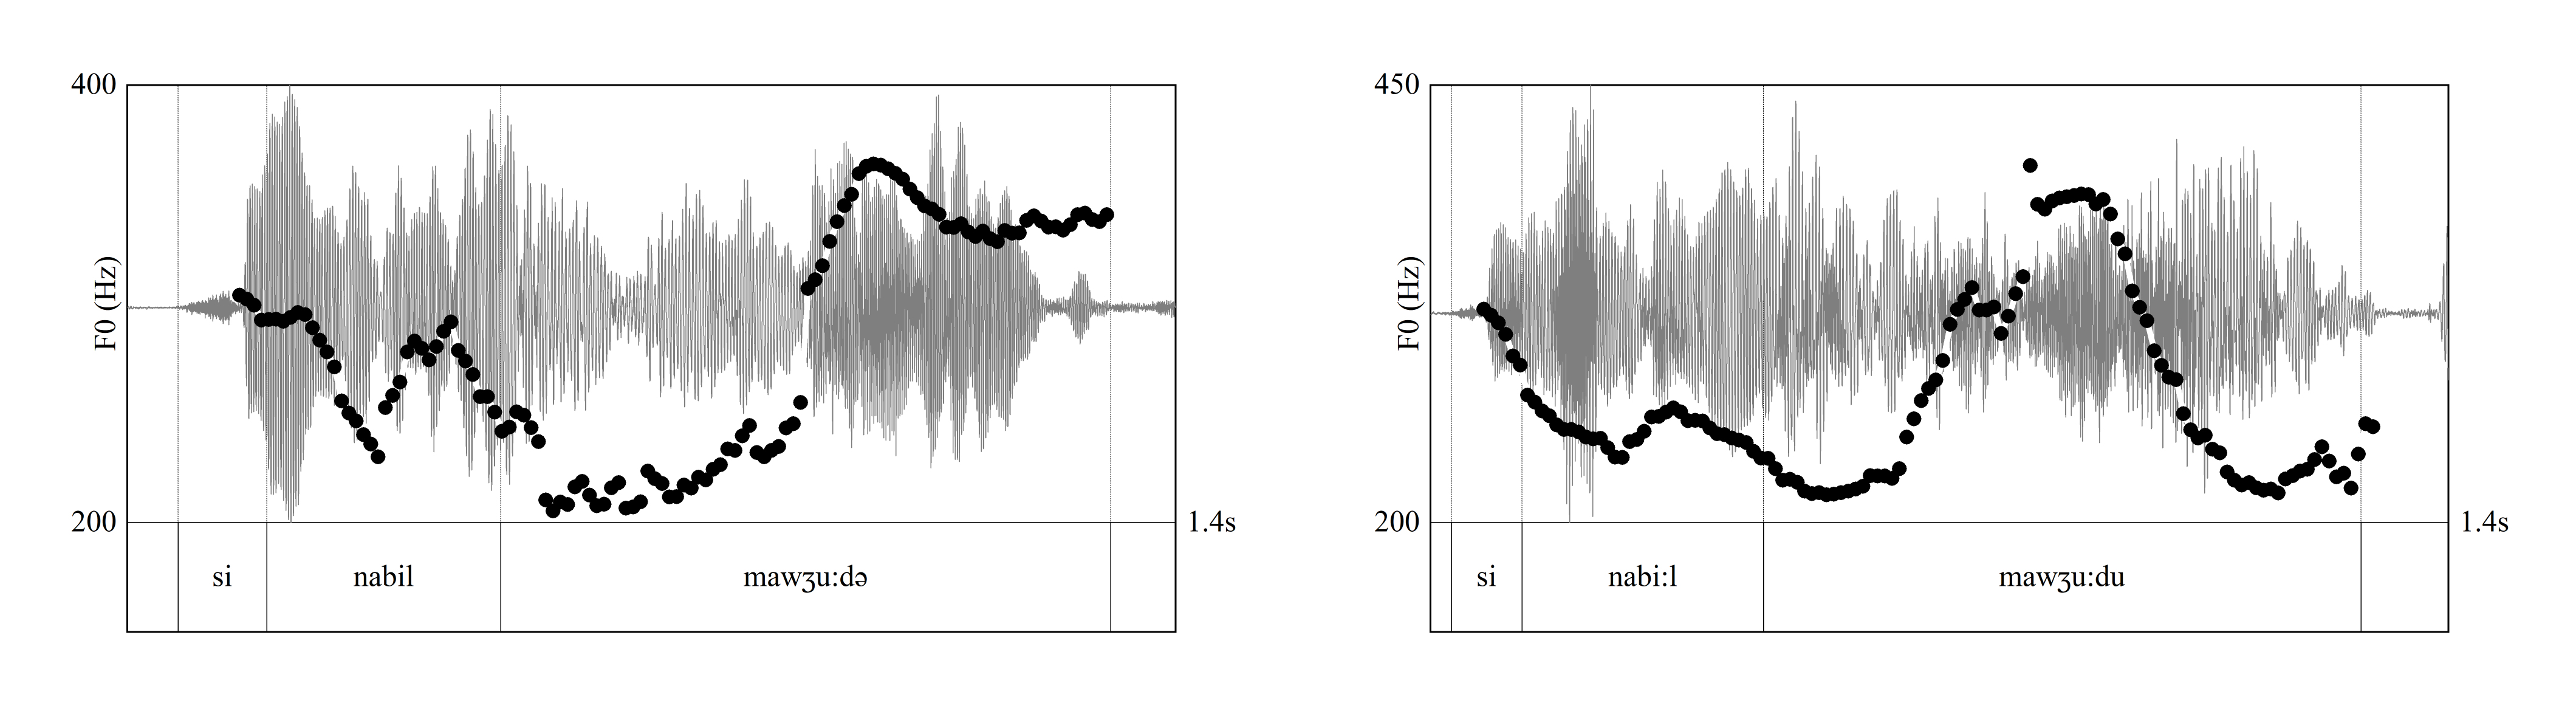
\includegraphics[width=\textwidth]{figures/intonation-img1.png}
\caption{\label{fig:key:1}Pitch trace of yes/no questions from a Tunisian Arabic speaker from Tunis (left) and from the southeast (right).}

\begin{tabularx}{\textwidth}{llX}
\lsptoprule
si & naˈbil & /mawˈʒud/ [mawˈʒudə/u]\\
Mr & Nabil & present\\
\multicolumn{3}{l}{‘Is Mr Nabil there?’  (tuno-arc1-f1/tuse-arc1-f1)}\\
\lspbottomrule
\end{tabularx}
\end{figure}

The rise--fall yes/no-question contour in TA differs from the rise seen in yes/no \isi{questions} in most \ili{Arabic} dialects \citep{Hellmuthtoappearbook} and, in terms of distribution, from the rise--fall contour observed in \ili{Moroccan} \ili{Arabic} (MA) across all utterance types (not only in yes/no \isi{questions}). The vowel \isi{epenthesis} marker appears to be unique to TA, thus far.

A pattern of utterance-final vowel \isi{epenthesis} has been observed in a number of \ili{Romance} languages spoken along the northern edge of the Mediterranean, including \ili{Bari} \ili{Italian} \citep{GriceEtAl2015}, and different varieties of \ili{Portuguese} \citep{FrotaEtAl2015}. These cases of utterance-final vowel \isi{epenthesis} are interpreted as text--tune adjustment, where segmental material is added to accommodate a complex prosodic contour.  For example, in \ili{Standard} European \ili{Portuguese}, a more general rule of utterance-final vowel deletion is blocked in utterances bearing a complex prosodic contour, such as the fall--rise (H+L* LH\%) on yes/no \isi{questions} \citep{FrotaEtAl2015}. In \ili{Bari} \ili{Italian}, \isi{epenthesis} is seen on a range of utterance types, but – like \ili{Portuguese} – its occurrence can be ascribed to tonal crowding (i.e. that the complex contour requires more segmental material to be realised). This is reflected in higher incidence of \isi{epenthesis} on utterance-final monosyllables than on longer words, and on words in which the final sound is an obstruent than on words with a final sonorant \citep{GriceEtAl2015}.

Investigation of utterance-final vowel \isi{epenthesis} in TA yes/no \isi{questions}, in a corpus of data collected in \ili{Tunis}, shows a very different pattern, however. In TA the incidence of \isi{epenthesis} is not affected by the number of syllables in the utterance-final word nor by the type of final sound. In addition, whereas in the other \ili{Romance} languages \isi{epenthesis} occurs on a range of utterance types, in TA \isi{epenthesis} occurs only in yes/no \isi{questions}, and predominantly in yes/no \isi{questions} which are produced with a complex rise--plateau or rise--fall contour \citep{Hellmuthforthcomingtunisianyesno}. The effects which in the \ili{Romance} languages are taken as evidence of text--tune adjustment are lacking in TA, which appears to rule out a language-internal (endogenous) source of the TA pattern of vowel \isi{epenthesis}.

The TA epenthetic vowel is in fact best characterized as an optional question marker comprising the vowel itself plus an accompanying fall in pitch. The segmental marker is well-known among \ili{Tunisian} linguists, being described as “the pan-\ili{Tunisian} question marker \isi{clitic} [ā]” (\citealt{HerinZammit2017}: 141), but the accompanying prosodic contour has received little attention in the literature until recently. This traditional question-marking strategy may however be in decline, since it now alternates with realisation of a yes/no question using a simple rise contour similar to that found in most other \ili{Arabic} dialects, and without an utterance-final epenthetic vowel. The picture is complicated by the fact that there is a somewhat higher incidence of \isi{epenthesis} among young female speakers, who might be expected to use the traditional form less, rather than more \citep{Hellmuthforthcomingtunisianyesno}. 

The \isi{epenthesis} + complex contour strategy in TA yes/no \isi{questions} stands out from other \ili{Arabic} dialects and may thus be due to contact-induced prosodic change. \ili{Italian} was spoken in Tunisia more widely than \ili{French}, in the late nineteenth century \citep{Sayahi2011}, and is thus a potential source of the contour, since rise--falls occur in yes/no \isi{questions} in a number of \ili{Italian} dialects \citep{GiliFivelaEtAl2015}. However, the conditioning environments of \isi{epenthesis} reported for \ili{Bari} \ili{Italian} are very different, suggesting that contact with \ili{Italian} is not a likely source of the \isi{epenthesis} component of the TA pattern.

An alternative source of the vowel \isi{epenthesis} pattern is \ili{French}, since Tunisia has seen very high levels of \isi{bilingualism} in TA and \ili{French} from the late nineteenth century up to the present day, despite concerted efforts to reduce usage of \ili{French} \citep{Daoud2007}. Utterance-final schwa \isi{epenthesis} has been reported as an emerging phenomenon in \ili{French} \citep{Hansen1997}, but its distribution is again much broader, being seen across a range of utterance types, and not restricted to yes/no \isi{questions}. Despite clear evidence of contact-induced effects of \ili{French} on TA in other domains, such as lexical borrowing, and a general trend towards use of \ili{French} by female speakers \citep{Walters2011}, the different distribution of final \isi{epenthesis} in \ili{French} suggests it is not the most likely source of the TA segmental question-marking strategy. 

The other major contact language with TA is \ili{Tunisian} \ili{Berber} (TB). Although levels of TA--\ili{Berber} \isi{bilingualism} in Tunisia are now low, other than in certain regions \citep{Gabsi2011}, there was a sustained period of TA--TB \isi{bilingualism} from the eleventh century, and TB is an important \isi{substrate} of TA \citep{Daoud2007}. Although there are no studies of the \isi{prosody} of TB, to our knowledge, a recent detailed study of \ili{Zwara} \ili{Berber}, spoken close to the \ili{Tunisian} border in western Libya, documents a polar question marking \isi{clitic} /a/ which is obligatorily accompanied by a rise--fall contour \citep{Gussenhoven2017}. The match of this description to the TA pattern is so close that it seems plausible that the TA question-marking pattern arose due to contact with TB during the period of sustained TA--TB \isi{bilingualism}. The greater use of the \isi{epenthesis} + contour strategy by female speakers than male speakers, as well as regional variation, makes this feature of TA ripe for further detailed sociolinguistic study.


 
 \subsection{Moroccan Arabic word prosody} \label{moroc}


Variation in word \isi{stress} patterns across \ili{Arabic} dialects has inspired much phonological investigation \citep{Watson2011stress}, but the \ili{Moroccan} \ili{Arabic} (MA) \isi{stress} system has defied analysis until recently. Mitchell (\citeyear[202]{Mitchell1993}) notes that “in contrast with all the other vernaculars […], the place of prominence in a word in isolation is not carried over to its occurrence in the phrase and sentence”, and this characterization was confirmed experimentally by \citet{Boudlal2001}. A range of positions have emerged, with some authors claiming that MA does have word \isi{stress} (\citealt{Benkirane1998}; \citealt{BurdinEtAl2014}), and others that it does not (\citealt{Maas2013}; \citealt{ElZarka2012}). 

It is now clear that MA is indeed typologically different from most other \ili{Arabic} dialects in its word \isi{prosody}. Whereas the majority of \ili{Arabic} dialects have salient word-level \isi{stress} and are thus clearly ``\isi{head-marking}'' languages, in the typology proposed by \citet{Jun2005}, MA is a non-\isi{head-marking} language in which tonal events mark the edges of prosodic phrases only. \citet{Bruggeman2018} provides acoustic evidence that there are no consistent cues to lexical prominence in MA, and perceptual evidence that MA listeners display the same type of ``\isi{deafness}'' to \isi{stress} as has been reported for listeners in languages which also lack head marking such as \ili{French} \citep{DupouxPeperkamp2001} and \ili{Persian} \citep{RahmaniRietveldGussenhoven2015}.

Can this stark variation in prosodic type between MA and other dialects of \ili{Arabic} be attributed to contact-induced change? The \ili{Arabic} language has been in sustained contact with \ili{Amazigh} (\ili{Moroccan} \ili{Berber}, MB) since the seventh century, but also with \ili{Latin}, \ili{French} and \ili{Spanish}\ia{Heath, Jeffrey@Heath, Jeffrey} (Heath, this volume). \citet{MaasProcházka2012} argue from corpus data that MA and MB share a common phonology, across a range of segmental and suprasegmental features. \citet{Bruggeman2018} confirms that there is no difference between MA and Tashlhiyt MB: both lack acoustic cues to word-level prominence in production and both groups of listeners display \isi{stress} \isi{deafness}. 

Since \ili{French} is also an edge-marking language, without lexical \isi{stress}, can we rule out \ili{French} as an alternative source of this prosodic feature of MA? The main evidence comes from the fact that MA and MB also share other prosodic features which are not found in \ili{French}, such as the shape of the tonal contour used to mark the edges of phrases, which is a rise in \ili{French} \citep{Delais-Roussarieetal2015}, but a rise--fall in both Tashlhiyt MB (\citealt{GriceEtAl2015,BruggemanRoettgerGrice2017}) and MA (\citealt{Benkirane1998,Hellmuthtoappearbook}). The contrast is also exemplified in Faygal's (\citeyear{Fagyal2005}) study of \ili{French}--MA bilinguals in Paris who use an MA rise--fall contour in \ili{French}.  


 
 \subsection{Egyptian Arabic accent distribution} \label{egypt}


\ili{Cairene} \ili{Egyptian} \ili{Arabic} (EA) displays a rich distribution of sentence accents, with a pitch accent typically observed on every content word. This has been noted independently by different authors (\citealt{Rifaat1991,Rastegar-ElZarka1997}), and is observed in both read and spontaneous speech styles \citep{Hellmuth2006}. Initial studies suggest that the same may be true also of some other dialects, such as Emirati \citep{BlodgettOwensRockwood2007} or \ili{Ḥiǧāzi} \citep{Alzaidi2014}, but these observations await corroboration across different speech styles. 

Dense \isi{accent distribution} has been noted in some languages on the northern coast of the Mediterranean also, including \ili{Spanish} and \ili{Greek}  \citep{Jun2005}, although, in \ili{Spanish}, the rich \isi{accent distribution} seen in laboratory speech is reduced in spontaneous speech \citep{Face2003}. \ili{Portuguese} dialects vary in \isi{accent distribution}: most varieties typically have an accent on every content word, but \ili{Standard} European \ili{Portuguese} shows an accent on the first and last words in an utterance only \citep{FrotaEtAl2015}. 

Rich \isi{accent distribution} is not observed in \ili{Moroccan} \ili{Arabic} \citep{Benkirane1998}, nor in \ili{Tunisian} \ili{Arabic} \citep{Hellmuthtoappearbook}. If the EA \isi{accent distribution} pattern were due to contact between EA and the southern European languages on the other side of the Mediterranean which share the tendency towards rich \isi{accent distribution}, we might expect the pattern to be found all across North Africa.

There is strong documentary evidence from written sources of historical sustained multilingualism in Egypt. \ili{Greek} arrived in Egypt in the fourth century BCE, serving as a formal administrative language alongside \ili{Egyptian} for several centuries, and with the country reaching a state of “balanced societal \isi{bilingualism}” in \ili{Greek} and \ili{Egyptian} in the sixth and seventh centuries CE \citep[6]{Papaconstantinou2010}. \ili{Egyptian} evolved into \ili{Coptic}, and its \isi{prestige} continued to increase from the sixth century CE onwards. After the Arab conquest in the seventh century CE, \ili{Arabic} began to take over from \ili{Greek} as the language of administration, eventually replacing \ili{Coptic} in daily use \citep{Papaconstantinou2012}. 

Is it possible that \ili{Egyptian}--\ili{Coptic} or \ili{Greek} is the source of the rich \isi{accent distribution} observed in EA (and indeed in \ili{Romance} languages in southern Europe)? 

The distribution of full and long vowels in \ili{Coptic} indicates that it had word-level prominence \citep[270]{Peust1999}, but it is not possible to determine from written texts the nature or distribution of any tonal contours which may have been associated with prominent syllables. Anecdotal evidence suggests that the \isi{intonation} patterns used in surviving liturgical forms of \ili{Coptic} are very different from those in EA \citep[32]{Peust1999}, though this difference may owe more to the liturgical setting than to properties of the languages in spoken form.

\ili{Ancient} \ili{Greek} is generally thought to have had a pitch accent system in which the primary marker of culminative accent in each word was pitch (\citealt{DevineStephens1985}). The \isi{Koine} \ili{Greek} dialect used in Egypt is thought to have lost pitch accent in favour of a \isi{stress} accent system, however, by the fourth century BCE \citep{Benaissa2012}. 

Support for the hypothesis that \ili{Greek} is the original source of the rich \isi{accent distribution} would come from a match between the historical spread of \isi{Koine} \ili{Greek} around the Mediterranean with the location of languages in which rich \isi{accent distribution} is also found. This would predict that eastern varieties of Libyan (Cyrenaican) \ili{Arabic} might also be found to display rich \isi{accent distribution}. If rich \isi{accent distribution} is confirmed in dialects of \ili{Arabic} (such as Emirati or \ili{Ḥiǧāzi}) which did not have sustained contact with \ili{Greek}, or with EA more recently, this would argue against \ili{Greek} as the original source. Although Nubi \citep{Gussenhoven2006} and \ili{Juba} \ili{Arabic} \citep{Nakao2013} display hybrid properties between \isi{stress} and lexical \isi{tone}, the most likely explanation of their prosodic patterns is direct contact with local tonal languages. A potential endogenous trigger for development of rich \isi{accent distribution} would be the absence of other forms of phonological marking of word domains, which are indeed somewhat reduced in EA, in comparison to other dialects \citep{Watson2002}, though the direction of causality of this correlation is not easily determined. 

Accent distribution has only recently been added to the parameters of variation explored in work on \isi{prosody} \citep{Hellmuth2007}, and thus included in descriptions of the \isi{intonation} systems of languages (e.g. \citealt{FrotaPrieto2015}). As further descriptions emerge of more dialects of \ili{Arabic} it will be important to include documentation of \isi{accent distribution}, across genres and speaking styles, in \isi{future} research.
\largerpage

\section{Conclusion} \label{closes}

There is much that we do not yet know about variation in \isi{intonation} in \ili{Arabic}, which leaves scope for investigation of further potential cases of contact-induced prosodic change. One such case may be the \ili{Syrian} \ili{Arabic} utterance-final rising \isi{intonation}, sometimes known as ``drawl'', which is found in yes/no \isi{questions} but also across other utterance types \citep{Cowell1964}, and which is an identifiable feature of the \ili{Damascus} dialect \citep{KulkOdéWoidich2003}. Although the full geographical range of the pattern has not been investigated in detail, and may be diffused to other dialects in the Levant, this rising declarative \isi{intonation} pattern stands out from most other \ili{Arabic} dialects, and is thus another potential case of contact-induced change. 

Another potential outlier pattern is the rise--fall \isi{intonation} contour seen in yes/no \isi{questions} in \ili{Yemeni} \ili{Arabic} from Ṣanʕāʔ \citep{Hellmuth2014}. The full areal reach of this prosodic question-marking strategy is also not yet fully known, and may extend into \ili{Ḥiǧāzi} \ili{Arabic} and western dialects of \ili{Oman}. However, we do know that a rise--fall is seen in both Tunisia and Morocco, though in these places the pattern may be due to contact with varieties of \ili{Amazigh} \ili{Berber}. Nevertheless, it is tempting to speculate how a pattern found in \isi{Yemen} might also be found in Tunisia and Morocco, and thus to explore the potential role of contact-induced variation due to ancient migrations between the eighth and fourteenth centuries \citep{Holes2018}.

Finally, the \isi{intonation} of \ili{Modern Standard} \ili{Arabic} (MSA) and of other formal registers may prove to be a fruitful domain of \isi{future} research. As our knowledge of the intonational phonology of spoken \ili{Arabic} dialects improves, this will facilitate investigation of the extent to which the \isi{intonation} patterns of a speaker’s regional dialect can be observed and/or perceived in their MSA speech, building on the findings of prior studies (\citealt{ElZarkaHellmuth2009}). An important goal would be to determine the extent to which a separate intonational system can be described for MSA, and to document the differential contribution to this system of specific genres of MSA discourse versus contact-induced influence due to widespread community mastery of multiple registers of the language.  

All these investigations would benefit from improved documentation of the time depth of present-day surface \isi{intonation} patterns. For the quasi-unique features explored in §\ref{araint}, we do not know whether these are the result of recent or much more distant historical change. This situation might be rectified through analysis of archive audio materials, though dialect studies have often worked on oral narratives, which yield only a limited range of prosodic expression (i.e. usually few \isi{questions}, and no information about turn-taking). A more viable strategy to gauge the time depth of contact-induced variation in \ili{Arabic} \isi{intonation} would be for \isi{future} sociolinguistic studies to include prosodic features as variables in apparent-time studies with participants in different age ranges, or for pre-existing corpora of apparent-time data to be made available for prosodic analysis.

\section*{Further reading}

There are two key reference works, so far, on \isi{intonation} in \ili{Arabic} dialects, based on secondary analysis of prior published work: \citet{Chahal2011} and \citet{ElZarka2017}. Hellmuth (\citeyear{Hellmuth2019}) suggests prosodic variables for inclusion in studies of variation and change in \ili{Arabic}. 

\section*{Acknowledgements}

The Intonational Variation in \ili{Arabic} corpus (\citealt{HellmuthAlmbark2017}) was funded by an award to the author by the UK Economic and Social Research Council (ES/I010106/1).

\section*{Abbreviations}
\setlength{\columnsep}{30pt}
\begin{multicols}{2}
\begin{tabbing}
\textsc{ipfv} \hspace{1em} \= before common era\kill
AM \> Autosegmental-Metrical theory \hspace{10mm} \\
BCE \> before Common Era \\
CE \> Common Era \\
EA \> \ili{Egyptian} \ili{Arabic} \\
H \> high \isi{tone} \\
L \> low \isi{tone} \\
L1, L2 \> 1st, 2nd language \\
MA \> \ili{Moroccan} \ili{Arabic} \\
MB \> \ili{Moroccan} \ili{Berber} \\
MSA \> \ili{Modern Standard} \ili{Arabic} \\
TA \> \ili{Tunisian} \ili{Arabic} \\
TB \> \ili{Tunisian} \ili{Berber} \\
YA \> \ili{Yemeni} \ili{Arabic}
\end{tabbing}
\end{multicols}

\sloppy
\printbibliography[heading=subbibliography,notkeyword=this]
\end{document}